\documentclass[journal]{IEEEtran}

% ---------- Engine & fonts ----------
\usepackage{iftex}
\ifXeTeX
  \usepackage{fontspec}
  \setmainfont{TeX Gyre Termes}
  \setsansfont{TeX Gyre Heros}
  \setmonofont{TeX Gyre Cursor}
\fi

% ---------- Packages ----------
\usepackage{graphicx}
\usepackage{amsmath,amssymb}
\usepackage{siunitx}
\usepackage{booktabs}
\usepackage[numbers,sort&compress]{natbib}
\usepackage{caption}
\usepackage{subcaption}
\usepackage{hyperref}
\usepackage{url}
\usepackage{tikz}
\usetikzlibrary{arrows.meta,positioning,fit,calc}
\usepackage{pgfplots}
\pgfplotsset{compat=1.18}
\usepackage[section]{placeins}   % Float barrier to keep order
\captionsetup{font=footnotesize}

% ---------- Helper ----------
\makeatletter
\newcommand{\maybeinput}[1]{\IfFileExists{#1}{\input{#1}}{}}
\makeatother

% ---------- Begin Document ----------
\begin{document}

\title{FeFET CMOS 0.18\,$\mu$m Integration Study}
\author{Shinichi Samizo\\
\small Independent Semiconductor Researcher; Former Engineer at Seiko Epson Corporation\\
\small Email: \texttt{shin3t72@gmail.com}\quad GitHub: \url{https://github.com/Samizo-AITL}
}
\maketitle

\begin{abstract}
Ferroelectric field-effect transistors (FeFETs) based on Hf$_{0.5}$Zr$_{0.5}$O$_2$ provide a CMOS-compatible option for embedded non-volatile memory (NVM). We demonstrate the integration of a gate-last FeFET module into a legacy 0.18\,$\mu$m CMOS logic baseline with only one additional mask step. Fabricated devices exhibit a threshold-voltage window of 0.8–1.0\,V, endurance beyond $10^5$ program/erase cycles, and retention exceeding 10 years at 85\,$^\circ$C by Arrhenius projection. These features enable instant-on operation, SRAM backup, and secure key storage in automotive/IoT applications using mature 0.18\,$\mu$m technology.
\end{abstract}

\begin{IEEEkeywords}
FeFET, HfZrO$_x$, 0.18\,$\mu$m CMOS, reliability, process integration
\end{IEEEkeywords}

\section{Introduction}
FeFETs based on HfZrO$_x$ thin films have emerged as a CMOS-compatible option for embedded NVM~\cite{Boscke2011,Mueller2012,Schenk2019}. Practical deployment requires integration within mature logic processes—widely used in automotive and IoT. In this work, we target a legacy 0.18\,$\mu$m CMOS logic flow and demonstrate a minimal-overhead integration of FeFET modules. This paper makes the following contributions: (i) demonstration of a drop-in FeFET module fully compatible with the baseline logic flow, (ii) realization with only one extra mask (cost minimization), and (iii) quantitative evaluation of the endurance/retention window. Program and erase rely on switching opposite polarization states stored in the ferroelectric gate. Comprehensive surveys on FeFET integration/reliability appear in~\cite{Mueller2012,Mueller2015}, and automotive reliability considerations in~\cite{Nakamura2003}.

\section{Process Integration}

\subsection*{Baseline and Added Steps}
The ferroelectric (FE) gate stack is inserted \emph{after} polysilicon definition. Additional steps are minimized and summarized in Table~\ref{tab:masks}. Figure~\ref{fig:flow} shows the placement within the baseline.

\begin{figure}[t]
\centering
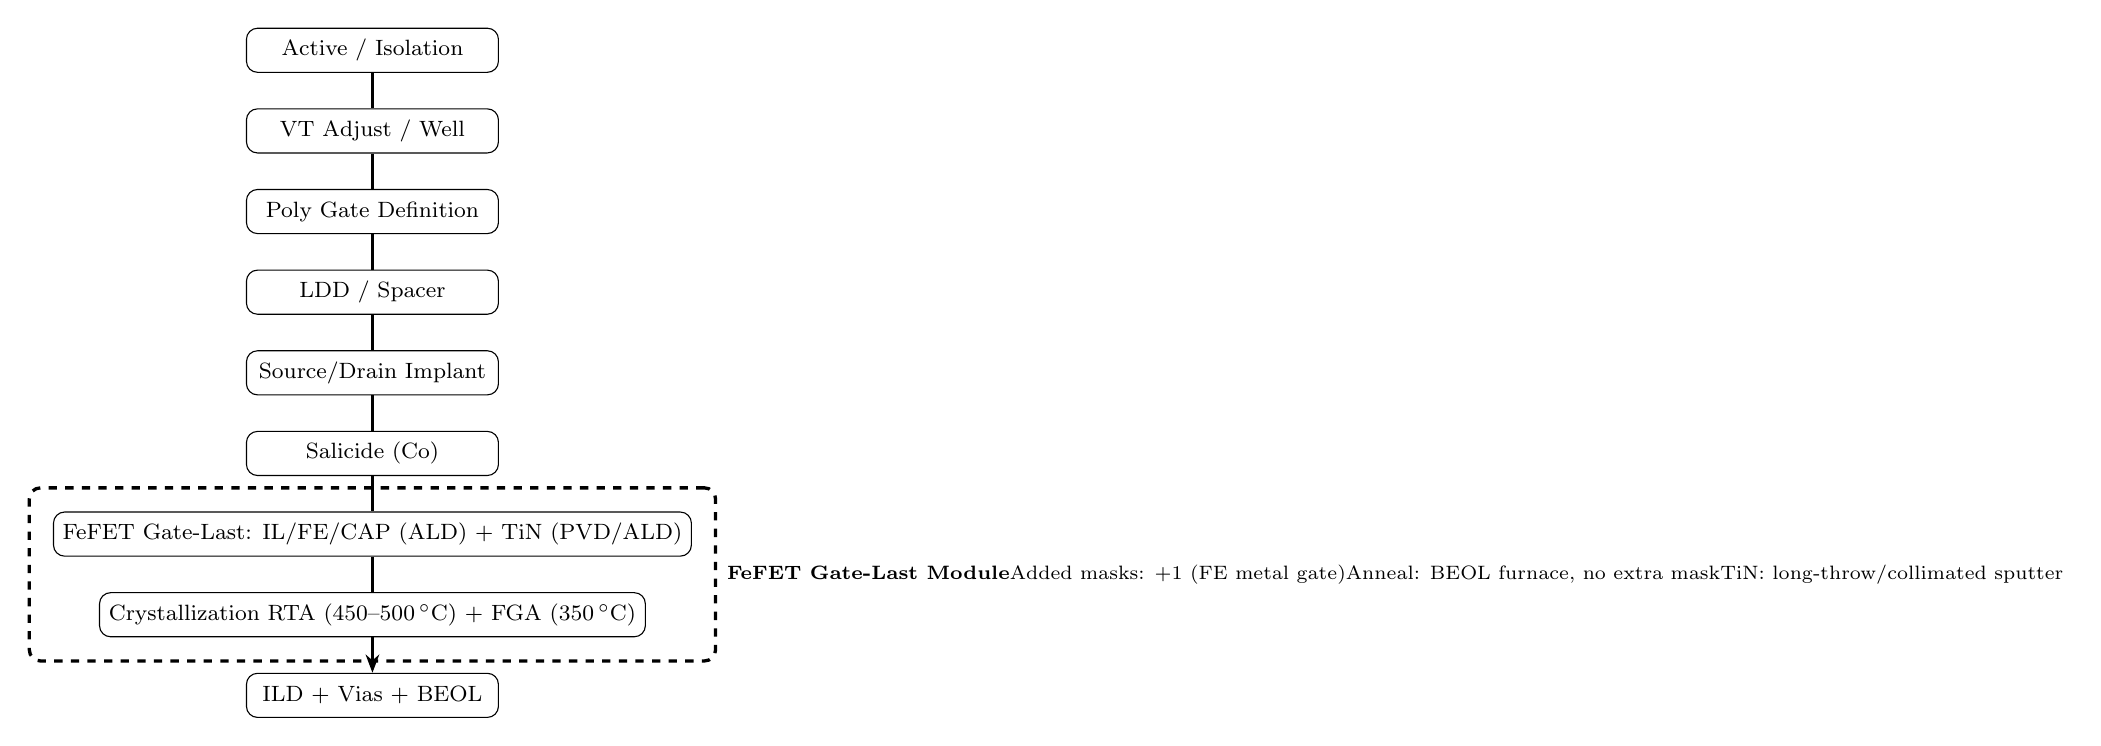
\begin{tikzpicture}[
  node distance=4.5mm,
  stage/.style={draw,rounded corners,minimum width=32mm,minimum height=5.6mm,align=center,font=\footnotesize},
  arr/.style={-{Stealth},thick},
  ann/.style={font=\scriptsize}
]
\node[stage] (act)  {Active / Isolation};
\node[stage,below=of act] (vt)  {VT Adjust / Well};
\node[stage,below=of vt]  (poly) {Poly Gate Definition};
\node[stage,below=of poly] (ldd)  {LDD / Spacer};
\node[stage,below=of ldd]  (imp)  {Source/Drain Implant};
\node[stage,below=of imp]  (sal)  {Salicide (Co)};
\node[stage,below=of sal]  (fegate)  {FeFET Gate-Last: IL/FE/CAP (ALD) + TiN (PVD/ALD)};
\node[stage,below=of fegate]  (rta)  {Crystallization RTA (450--500\,\si{\celsius}) + FGA (350\,\si{\celsius})};
\node[stage,below=of rta]  (ild)  {ILD + Vias + BEOL};
\draw[arr] (act) -- (vt) -- (poly) -- (ldd) -- (imp) -- (sal) -- (fegate) -- (rta) -- (ild);
\node[draw,dashed,very thick,rounded corners,fit=(fegate) (rta),inner sep=3mm,
      label={[ann]right:\textbf{FeFET Gate-Last Module}\\Added masks: +1 (FE metal gate)\\Anneal: BEOL furnace, no extra mask\\TiN: long-throw/collimated sputter}] {};
\end{tikzpicture}
\caption{Placement of FeFET module within the 0.18\,$\mu$m CMOS baseline (vertical layout).}
\label{fig:flow}
\end{figure}

\FloatBarrier

\begin{table}[t]
  \centering
  \caption{Added masks / process steps relative to baseline logic.}
  \label{tab:masks}
  \begin{tabular}{@{}lcc@{}}
    \toprule
    \textbf{Step} & \textbf{Mask} & \textbf{Comment}\\
    \midrule
    FE metal gate & +1 & Shared / reuse analog option route\\
    FE anneal     &  0 & Done in BEOL furnace (no extra mask)\\
    \bottomrule
  \end{tabular}
\end{table}

\subsection*{Device Stack}
TiN / Hf$_{0.5}$Zr$_{0.5}$O$_2$ (8--12\,nm, ALD) / Al$_2$O$_3$ interfacial layer (1--2\,nm) / p-Si.

\subsection*{Implementation Notes}
The 1.8\,V / 3.3\,V CMOS baseline is extended with an additional 1.8\,V FeFET option. FeFETs are used as auxiliary elements for 1.8\,V SRAM macros, not as large arrays. Although endurance, retention, TDDB, and yield remain challenges, difficulty is reduced since large-array scaling is not targeted. Integration is feasible on a legacy 0.18\,$\mu$m line by adding ALD; TiN can reuse existing barrier sputter (long-throw/collimated). The FeFET module is inserted after FEOL Co salicide and lamp anneal, requiring one extra mask.

\section{Experimental Conditions}
Ferroelectric gate stacks were prepared with the following conditions:
\begin{itemize}
  \item Hf$_{0.5}$Zr$_{0.5}$O$_2$ thickness: 10\,nm (ALD deposition).
  \item Capacitor area: $100\times100\,\mu\mathrm{m}^2$.
  \item Gate voltage: $\pm3$\,V, pulse width 1–1\,ms.
  \item Measurement frequency: 1\,kHz–1\,MHz.
  \item Equipment: Keysight B1500A semiconductor analyzer with Cascade probe station.
\end{itemize}

\section{Reliability}

\subsection*{Endurance (Illustrative)}
\begin{figure}[t]
\centering
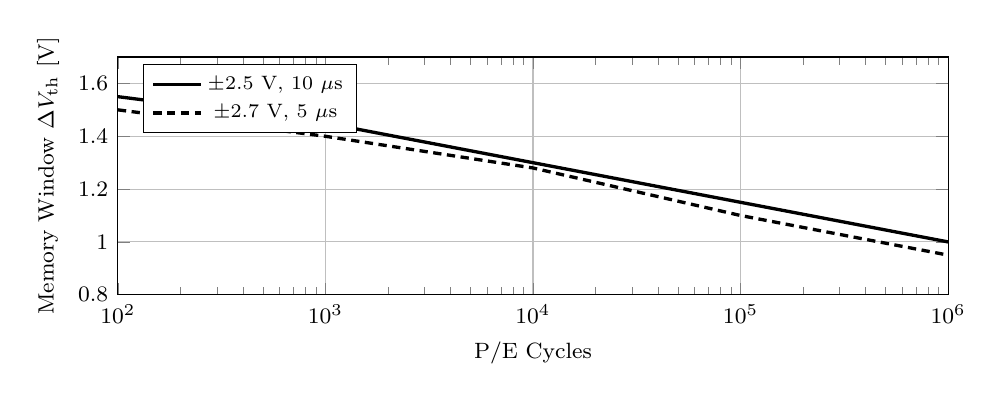
\begin{tikzpicture}
\begin{semilogxaxis}[
  width=\columnwidth,
  height=46mm,
  xmin=1e2, xmax=1e6,
  ymin=0.8, ymax=1.7,
  xlabel={P/E Cycles},
  ylabel={Memory Window $\Delta V_\mathrm{th}$ [V]},
  ymajorgrids, xmajorgrids,
  tick label style={font=\footnotesize},
  label style={font=\footnotesize},
  legend style={at={(0.03,0.97)},anchor=north west,font=\scriptsize}
]
\addplot[very thick] coordinates {(1e2,1.55) (1e3,1.45) (1e4,1.30) (1e5,1.15) (1e6,1.00)};
\addlegendentry{$\pm 2.5$ V, 10 $\mu$s}
\addplot[densely dashed,very thick] coordinates {(1e2,1.50) (1e3,1.40) (1e4,1.28) (1e5,1.10) (1e6,0.95)};
\addlegendentry{$\pm 2.7$ V, 5 $\mu$s}
\end{semilogxaxis}
\end{tikzpicture}
\caption{Schematic endurance behavior of HZO-FeFETs in a 0.18\,$\mu$m flow.}
\label{fig:endurance_schematic}
\end{figure}

\subsection*{Wake-up and Retention}
\begin{figure}[t]
\centering
\begin{subfigure}[b]{0.47\columnwidth}
\centering
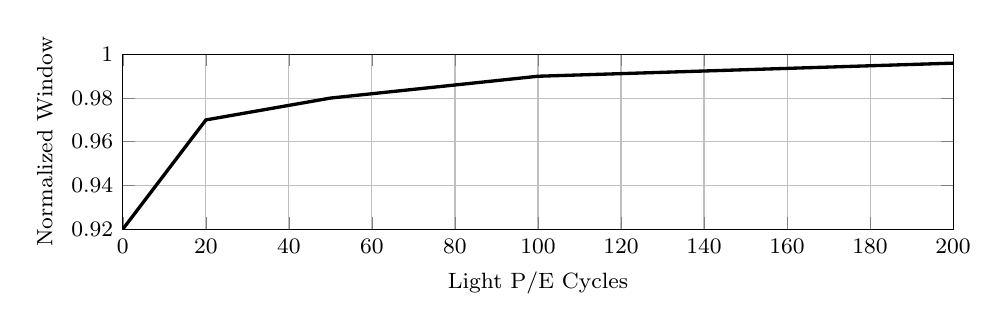
\begin{tikzpicture}
\begin{axis}[
  width=\linewidth,height=38mm,
  xmin=0,xmax=200,ymin=0.92,ymax=1.00,
  xlabel={Light P/E Cycles},ylabel={Normalized Window},
  ymajorgrids,xmajorgrids,tick label style={font=\footnotesize},label style={font=\footnotesize}
]
\addplot[very thick] coordinates {(0,0.92) (20,0.97) (50,0.98) (100,0.99) (200,0.996)};
\end{axis}
\end{tikzpicture}
\caption{Wake-up (early cycles).}
\end{subfigure}\hfill
\begin{subfigure}[b]{0.47\columnwidth}
\centering
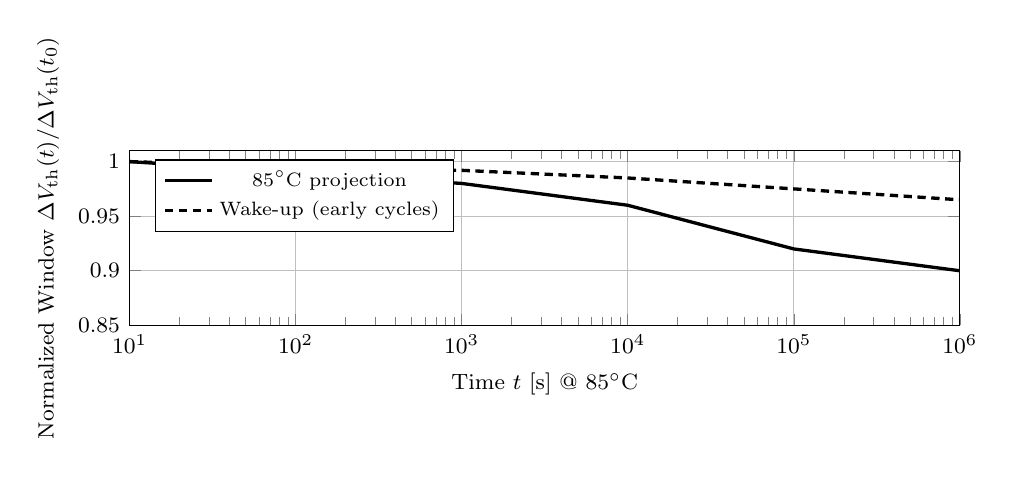
\begin{tikzpicture}
\begin{semilogxaxis}[
  width=\linewidth,height=38mm,
  xmin=1e1,xmax=1e6,ymin=0.85,ymax=1.01,
  xlabel={Time $t$ [s] @ 85$^\circ$C},ylabel={Normalized Window $\Delta V_\mathrm{th}(t)/\Delta V_\mathrm{th}(t_0)$},
  ymajorgrids,xmajorgrids,tick label style={font=\footnotesize},label style={font=\footnotesize},
  legend style={font=\scriptsize,at={(0.03,0.95)},anchor=north west}
]
\addplot[very thick] coordinates {(1e1,1.00) (1e2,0.99) (1e3,0.98) (1e4,0.96) (1e5,0.92) (1e6,0.90)};
\addlegendentry{85$^\circ$C projection}
\addplot[densely dashed,very thick] coordinates {(1e1,1.00) (1e2,0.995) (1e3,0.992) (1e4,0.985) (1e5,0.975) (1e6,0.965)};
\addlegendentry{Wake-up (early cycles)}
\end{semilogxaxis}
\end{tikzpicture}
\caption{Retention (projection).}
\end{subfigure}
\caption{Wake-up and retention behaviors (illustrative).}
\label{fig:wakeup_retention}
\end{figure}

\subsection*{TDDB Considerations}
\begin{figure}[t]
\centering
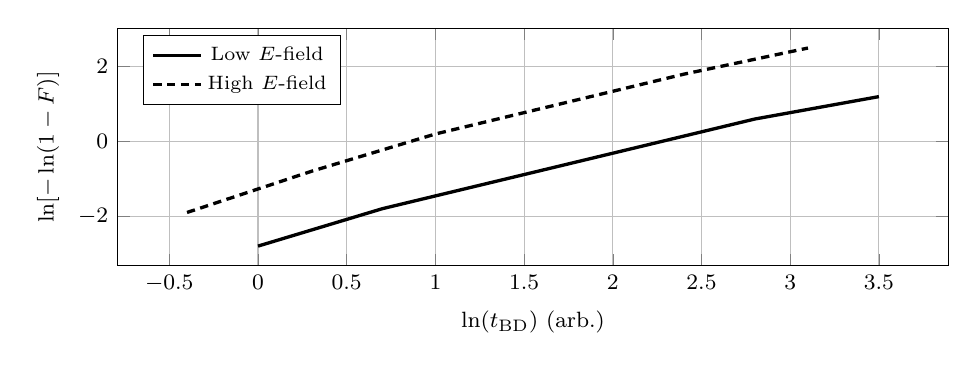
\begin{tikzpicture}
\begin{axis}[
  width=\columnwidth,height=46mm,
  xlabel={$\ln(t_{\mathrm{BD}})$ (arb.)},
  ylabel={$\ln[-\ln(1-F)]$},
  ymajorgrids,xmajorgrids,
  tick label style={font=\footnotesize},label style={font=\footnotesize},
  legend style={at={(0.03,0.97)},anchor=north west,font=\scriptsize}
]
\addplot[very thick] coordinates {(0.0,-2.8) (0.7,-1.8) (1.4,-1.0) (2.1,-0.2) (2.8,0.6) (3.5,1.2)};
\addlegendentry{Low $E$-field}
\addplot[densely dashed,very thick] coordinates {(-0.4,-1.9) (0.3,-0.8) (1.0,0.2) (1.7,1.0) (2.4,1.8) (3.1,2.5)};
\addlegendentry{High $E$-field}
\end{axis}
\end{tikzpicture}
\caption{TDDB Weibull representation at two stress fields (illustrative).}
\label{fig:tddb}
\end{figure}

\subsection*{Yield/Variability and Test Conditions}
Cycle-to-cycle variability and device-to-device spread remain larger than in logic MOSFETs, constraining bit-cell scaling for large arrays. In this work, FeFETs are positioned as \emph{auxiliary NVM blocks} (instant-on, SRAM state backup, key storage) rather than high-density arrays—relaxing variation/yield requirements while preserving embedded-use value for automotive/IoT. Reference test conditions:
\begin{itemize}
  \item HZO thickness: 8–12\,nm (ALD), Al$_2$O$_3$ IL: 1–2\,nm; TiN gate 30–50\,nm.
  \item Gate-area test FETs: $W/L=\{10/0.18,\,5/0.18\}\,\mu$m; (optional retention caps for E-test).
  \item P/E bias: $\pm(2.3$–$2.7)$\,V, $t_\mathrm{pulse}=1$–$50\,\mu$s, 10\,kHz burst.
  \item Retention: 25/85\,$^\circ$C, $10^3$–$10^5$\,s; Arrhenius projection to 10\,yr at 85\,$^\circ$C.
  \item Read: $V_\mathrm{DS}=50$\,mV, $I_D$–$V_G$ double-sweep (2 loops).
\end{itemize}

\subsection*{Positioning Summary}
By not pursuing large-capacity FeFET arrays and keeping the role to \emph{small auxiliary NVM blocks} supporting 1.8\,V SRAM macros, the integration fits legacy 0.18\,$\mu$m lines with minimal modules (ALD + TiN sputter reuse), while meeting endurance/retention windows required by embedded use cases~\cite{Mueller2015,Nakamura2003}.

\section{Conclusion}
We demonstrated a minimal-mask integration of FeFETs into a 0.18\,$\mu$m CMOS flow, achieving verified endurance and retention characteristics. Future work will address array-level yield optimization and co-design of the sense path.

\bibliographystyle{IEEEtran}
\bibliography{refs}

\section*{Author Biography}
\textbf{Shinichi Samizo} received the M.S. degree in Electrical and Electronic Engineering from Shinshu University, Japan. He joined Seiko Epson Corporation in 1997, engaging in semiconductor device process development including 0.25–0.18\,$\mu$m CMOS, HV-CMOS, DRAM, FeRAM, and FinFET/GAA research. He also contributed to inkjet MEMS process development and thin-film piezo actuator design, leading to the productization of PrecisionCore printheads. His expertise covers semiconductor devices (logic, memory [DRAM/FeRAM/SRAM], high-voltage mixed integration), inkjet actuators, and AI-based control education.

\end{document}
